% !TEX program = xelatex
% 大学物理期中复习题：紧凑题库排版，短公式和横线均在题干内；全部原图由 TikZ 绘制。
% 编译方法：xelatex 大物期中复习题_重绘版.tex （运行两遍以稳定页码）
\documentclass[12pt,a4paper,UTF8]{ctexart}
\usepackage{fontspec}
\usepackage{amsmath,amssymb}
\usepackage{geometry}
\usepackage{tikz}
\usetikzlibrary{arrows.meta,decorations.pathmorphing,patterns,calc}
\usepackage{enumitem}
\usepackage{needspace}
\usepackage{fancyhdr}
\usepackage{microtype}
\usepackage{array}
\geometry{top=1.35cm,bottom=1.5cm,left=1.3cm,right=1.3cm,headheight=14pt,headsep=0.40cm,footskip=0.65cm}
\IfFontExistsTF{Times New Roman}{\setmainfont{Times New Roman}}{\setmainfont{Tinos}}
\IfFontExistsTF{Songti SC}{\setCJKmainfont{Songti SC}}{\setCJKmainfont{Noto Serif CJK SC}} % macOS 优先宋体，其他系统用 Noto Serif CJK SC
\ctexset{section={format=\large\bfseries,beforeskip=1.0ex,afterskip=0.6ex}}
\setlength{\parindent}{2em}
\setlength{\parskip}{0.18em}
\linespread{1.14}
\raggedbottom
\setlist[enumerate]{topsep=2pt,itemsep=1.5pt,parsep=0pt,leftmargin=2.5em}
\pagestyle{fancy}
\fancyhf{}
\fancyhead[L]{\small 大学物理期中复习题}
\fancyhead[R]{\small 题目整理版 · 图形重绘}
\fancyfoot[C]{\thepage}
\renewcommand{\headrulewidth}{0.35pt}
\newcommand{\qitem}[1]{\par\needspace{5\baselineskip}\smallskip\noindent\textbf{#1}\hspace{0.5em}}
% 直接嵌在正文或行内数学环境中的答题横线，不另起行
\newcommand{\fillblank}[1][2.6cm]{\rule[-0.48ex]{#1}{0.45pt}}
\newcommand{\tfbox}{\ensuremath{[\quad\quad]}}
\newcommand{\smallgap}{\vspace{0.15em}}
% 普通示意图独立居中，但不使用 display math，也不额外增加大段空白
\newenvironment{compactfigure}{\par\vspace{0.15em}\begingroup\centering}{\par\endgroup\vspace{0.10em}}
\newcommand{\sourcepage}[1]{\par\medskip\noindent{\small\bfseries 原稿第 #1 页}\par\vspace{-0.2em}\hrule\smallskip}
\begin{document}
\begin{center}
{\LARGE\bfseries 大学物理期中复习题}\par\vspace{0.25em}
{\small 扫描资料文字整理与示意图矢量重绘版（不含作答批注）}
\end{center}
\vspace{-0.55em}

\sourcepage{1}
\qitem{24.}在驻波中，当各质元运动到其平衡位置时，则 \tfbox
\begin{enumerate}[label=\Alph*.,leftmargin=2.3em]
\item 各质元的势能为零，驻波能量为零
\item 各质元的动能为零，驻波能量为零
\item 各质元的动能为零，驻波的能量为势能，能量集中在波节附近
\item 各质元的势能为零，驻波的能量为动能，能量集中在波腹附近
\end{enumerate}

\qitem{25.}扬声器与观察者均以 $100\,\mathrm{m/s}$ 恒速向墙面运动，扬声器发出的声波频率为 $2.00\,\mathrm{kHz}$。若空气中声速为 $343\,\mathrm{m/s}$，则观察者接收到墙面反射的声波频率是 \tfbox
\par\noindent\hspace*{1.5em}\textbf{A.}\ $3.65\,\mathrm{kHz}$\qquad \textbf{B.}\ $2.82\,\mathrm{kHz}$\qquad \textbf{C.}\ $2.58\,\mathrm{kHz}$\qquad \textbf{D.}\ $2.00\,\mathrm{kHz}$

\qitem{5.（3 分）}在 $z$ 轴的原点 $O$ 处（$z=0$）有一平面波波源，其运动方程为 $\psi(t)=A\cos(\omega t)$，其中 $A$ 和 $\omega$ 为已知常量。波源产生的波沿 $z$ 轴正方向传播（设介质无吸收），波长为 $\lambda$。此波在 $z=L$（$L>0$）处发生反射。若反射点为固定端，反射波和入射波的振幅相等，写出反射波的波函数表达式。
\vspace{0.22cm}

\noindent\textbf{判断题（原稿第 1 页）}\quad 在括号内判断正误。
\begin{enumerate}[label=\arabic*.,leftmargin=2.3em]
\item 一切与热现象有关的实际宏观过程都是不可逆过程。\tfbox
\item 系统经历任一可逆过程的熵变一定为零。\tfbox
\item 系统经历任一不可逆循环的熵变一定为零。\tfbox
\item 制冷机的制冷系数一定小于 $1$。\tfbox
\item 系统的热容值不可能为负。\tfbox
\end{enumerate}

\qitem{21.}如图所示，一定量的理想气体从体积为 $V_0$ 的平衡态 I 变化到体积为 $2V_0$ 的平衡态 II，气体处在态 I 和 II 时的压强均为 $p_0$。那么不管该气体经历怎样的热力学过程，以下三种说法：（1）气体对外做正功 $A>0$；（2）气体从外界吸收热量 $Q>0$；（3）气体的内能增大 $\Delta U>0$；总是正确的是 \tfbox。
\begin{compactfigure}
\begin{tikzpicture}[x=0.92cm,y=0.82cm,>=Stealth, every node/.style={font=\small}]
  \draw[->,thick] (0,0)--(4.6,0) node[right] {$V$};
  \draw[->,thick] (0,0)--(0,3.25) node[above] {$p$};
  \node[below left] at (0,0) {$O$};
  \draw[dashed,thin] (0,1.85)--(3.25,1.85);
  \draw[dashed,thin] (1.55,0)--(1.55,1.85);
  \draw[dashed,thin] (3.25,0)--(3.25,1.85);
  \fill (1.55,1.85) circle(1.8pt) node[above] {I};
  \fill (3.25,1.85) circle(1.8pt) node[above] {II};
  \node[left] at (0,1.85) {$p_0$};
  \node[below] at (1.55,0) {$V_0$};
  \node[below] at (3.25,0) {$2V_0$};
\end{tikzpicture}
\end{compactfigure}
\noindent\textbf{A.}（1）、（2）\qquad \textbf{B.}（2）、（3）\qquad \textbf{C.}（1）、（2）、（3）\qquad \textbf{D.}（3）

\qitem{2.（8 分）}某理想气体（比热容比为 $\gamma$）的可逆热机工作在温度分别为 $T_{\mathrm H}$ 和 $T_{\mathrm L}$ 的高、低温热源之间。具体循环过程如下：此理想气体先从体积 $V_1$ 等温膨胀到体积 $V_2$，再绝热膨胀到体积 $V_3$，接着等温压缩到体积 $V_4$，最后绝热压缩到体积 $V_1$。
\begin{enumerate}[label=\arabic*)]
\item 证明：$\displaystyle\frac{V_2}{V_1}=\frac{V_3}{V_4}$；
\item 求此热机效率 $\eta$（写出推导过程）；
\item 画出此循环的温熵示意图（$T$--$S$ 图），并在图中标出循环的方向。
\end{enumerate}
\vspace{0.16cm}

\sourcepage{2}
\qitem{4.（7 分）}如图所示，同一个介质中的两个相干波源 $S_1$ 和 $S_2$ 位于 $z$ 轴上，它们的坐标分别是 $0\,\mathrm m$ 和 $14.5\,\mathrm m$。它们激起的平面简谐波沿 $z$ 轴传播，波长 $\lambda$ 为 $8\,\mathrm m$，振幅 $A$ 均为 $0.1\,\mathrm m$。波源 $S_1$ 的初相位 $\varphi_{10}$ 和波源 $S_2$ 的初相位 $\varphi_{20}$ 相差 $\pi/8$，即 $\varphi_{10}-\varphi_{20}=\pi/8$。
\begin{compactfigure}
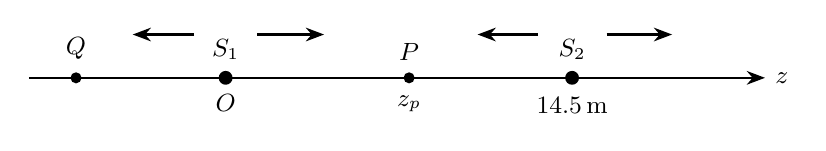
\begin{tikzpicture}[x=1cm,y=1cm,>=Stealth,every node/.style={font=\small}]
  \draw[->,thick] (-0.25,0)--(9.1,0) node[right] {$z$};
  \fill (0.35,0) circle(2pt) node[above=0.11cm] {$Q$};
  \fill (2.25,0) circle(2.5pt) node[above=0.11cm] {$S_1$} node[below=0.09cm] {$O$};
  \fill (4.58,0) circle(2pt) node[above=0.10cm] {$P$} node[below=0.10cm] {$z_p$};
  \fill (6.65,0) circle(2.5pt) node[above=0.11cm] {$S_2$};
  \node[below=0.12cm] at (6.65,0) {$14.5\,\mathrm m$};
  \draw[->,thick] (1.85,0.55)--(1.07,0.55);
  \draw[->,thick] (2.65,0.55)--(3.5,0.55);
  \draw[->,thick] (6.22,0.55)--(5.45,0.55);
  \draw[->,thick] (7.09,0.55)--(7.92,0.55);
\end{tikzpicture}
\end{compactfigure}
\begin{enumerate}[label=\arabic*)]
\item 设波源 $S_1$ 和 $S_2$ 连线上的 $P$ 点的坐标为 $z_p$（$0<z_p<14.5\,\mathrm m$），求波源 $S_1$ 和 $S_2$ 所发出的两列波在 $P$ 点所引起的振动的相位差 $\varphi_1-\varphi_2$。
\item 在波源 $S_1$ 和 $S_2$ 之间（$0<z_p<14.5\,\mathrm m$）的连线上有几个点由于干涉而静止？求出它们的位置坐标值（写出具体的坐标值）。
\end{enumerate}

\qitem{5.（3 分）}一定量的氮气（视为理想气体），从同一状态分别经历以下两种准静态过程：等压过程和等温过程，使氮气的体积由 $V_1$ 膨胀到 $3V_1$。若上述的等压过程和等温过程中氮气从外界吸收的热量分别为 $Q_p$ 和 $Q_T$，则 $Q_p:Q_T=\fillblank[3cm]$。

\qitem{6.（4 分）}物质的量为 $1\,\mathrm{mol}$ 的氮气（视为理想气体）向真空做绝热自由膨胀过程。设初状态气体的压强、体积分别为 $p_1$ 和 $V_1$，末状态气体的压强、体积为 $p_2$ 和 $V_2$。若气体体积膨胀为原来的 $3$ 倍（$V_2=3V_1$），则 $p_1:p_2=\fillblank[2.2cm]$；此过程气体熵的增量 $\Delta S=\fillblank[3cm]$。（摩尔气体常量为 $R$。）

\qitem{7.（3 分）}一理想可逆卡诺热机的高温热源温度为 $750\,\mathrm K$，低温热源温度为 $300\,\mathrm K$，每次循环向低温热源放出的热量为 $400\,\mathrm J$，则该热机的效率为 $\fillblank[2.4cm]$，每次循环可向外做功 $\fillblank[2.4cm]\,\mathrm J$。

\qitem{10.（3 分）}一质量为 $m$ 的滑块，两边分别与弹性系数为 $k_1$ 和 $k_2$ 的轻弹簧相连，两弹簧的另外一端分别固定在竖直墙面上。滑块可在光滑的水平面上滑动，$O$ 点为系统平衡位置。建立如图所示的坐标系，将滑块向右移动到 $x_0$ 处，自静止释放，并从释放时开始计时，则系统的运动方程为 $x=\fillblank[4cm]$。
\begin{compactfigure}
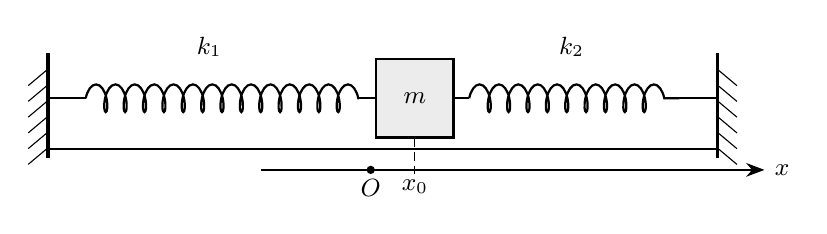
\begin{tikzpicture}[x=1.0cm,y=1cm,>=Stealth,every node/.style={font=\small}]
  \draw[very thick] (0,0)--(0,1.33) (8.5,0)--(8.5,1.33);
  \foreach \y in {0.05,0.25,...,1.20}{
    \draw[thin] (-0.25,\y-0.13)--(0,\y+0.08);
    \draw[thin] (8.5,\y+0.08)--(8.75,\y-0.13);
  }
  \draw[thick] (0,0.12)--(8.5,0.12);
  \draw[thick] (0,0.76)--(0.48,0.76);
  \draw[thick,decorate,decoration={coil,aspect=0.4,segment length=7pt,amplitude=5pt}] (0.48,0.76)--(3.95,0.76);
  \draw[thick] (3.95,0.76)--(4.17,0.76);
  \draw[thick,fill=gray!15] (4.17,0.26) rectangle (5.15,1.26);
  \node at (4.66,0.76) {$m$};
  \draw[thick] (5.15,0.76)--(5.35,0.76);
  \draw[thick,decorate,decoration={coil,aspect=0.4,segment length=7pt,amplitude=5pt}] (5.35,0.76)--(8.02,0.76);
  \draw[thick] (8.02,0.76)--(8.5,0.76);
  \node[above=0.40cm] at (2.05,0.76) {$k_1$};
  \node[above=0.40cm] at (6.65,0.76) {$k_2$};
  \draw[->,thick] (2.7,-0.15)--(9.1,-0.15) node[right] {$x$};
  \fill (4.10,-0.15) circle(1.5pt) node[below] {$O$};
  \draw[densely dashed,thin] (4.66,0.25)--(4.66,-0.22);
  \node[below] at (4.66,-0.15) {$x_0$};
\end{tikzpicture}
\end{compactfigure}

\qitem{14.（3 分）}右图为沿 $z$ 轴负方向传播的平面简谐波（波的周期为 $T$）在 $t=T/6$ 时的波形图，则原点（$z=0$）处的质点的振动的初相位为 $\fillblank[3cm]$。
\begin{compactfigure}
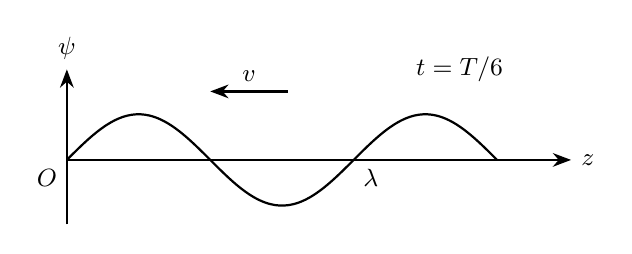
\begin{tikzpicture}[x=1.16cm,y=1cm,>=Stealth,every node/.style={font=\small}]
  \draw[->,thick] (0,-0.82)--(0,1.15) node[above] {$\psi$};
  \draw[->,thick] (0,0)--(5.52,0) node[right] {$z$};
  \node[below left] at (0,0) {$O$};
  \draw[thick,smooth,variable=\t,domain=0:4.71,samples=100] plot ({\t},{0.58*sin(114.65*\t)});
  \node[below right] at (3.14,0) {$\lambda$};
  \draw[->,thick] (2.42,0.87)--(1.57,0.87) node[midway,above] {$v$};
  \node[above] at (4.30,0.87) {$t=T/6$};
\end{tikzpicture}
\end{compactfigure}

\qitem{15.（4 分）}设声波在某介质中的传播速度为 $u$，声源 $S$ 的频率为 $f_s$。如图所示，声源 $S$ 和接收器 $R$ 沿着相同方向运动，它们相对于介质的速率分别为 $v_S$ 和 $v_R$（$v_R<v_S<u$）。位于 $S$ 和 $R$ 连线上的 $P$ 点处的介质质元的振动频率为 $\fillblank[3cm]$，接收器 $R$ 接收到的声波的频率为 $\fillblank[3cm]$。
\begin{compactfigure}
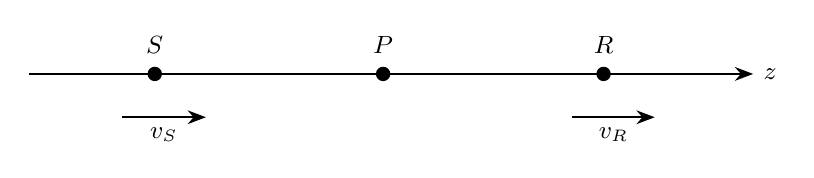
\begin{tikzpicture}[x=1cm,y=1cm,>=Stealth,every node/.style={font=\small}]
  \draw[->,thick] (0,0)--(9.2,0) node[right] {$z$};
  \fill (1.6,0) circle(2.6pt) node[above=0.13cm] {$S$};
  \fill (4.5,0) circle(2.6pt) node[above=0.13cm] {$P$};
  \fill (7.3,0) circle(2.6pt) node[above=0.13cm] {$R$};
  \draw[->,thick] (1.18,-0.55)--(2.25,-0.55) node[midway,below] {$v_S$};
  \draw[->,thick] (6.90,-0.55)--(7.95,-0.55) node[midway,below] {$v_R$};
\end{tikzpicture}
\end{compactfigure}

\sourcepage{3}
\qitem{1.（4 分）}如图所示，绝热气缸内有一个不导热的隔板把气缸分为 $A$、$B$ 两室，隔板可在气缸内无摩擦地平移，每室中有质量相同的同种单原子分子理想气体。如图（a）所示，开始时它们都处于压强为 $p_0$、体积为 $V_0$ 和温度为 $T_0$ 的状态。今通过电热丝传给 $A$ 室气体热量 $Q$，平衡时 $A$ 室体积为 $B$ 室的两倍（即 $A$ 室体积 $V_A=4V_0/3$），如图（b）所示，求：
\begin{compactfigure}
\begin{tikzpicture}[x=1cm,y=1cm, every node/.style={font=\small}]
  % （a）隔板在中点
  \fill[pattern=dots,pattern color=gray!55] (0.12,1.94) rectangle (3.08,3.38);
  \fill[pattern=dots,pattern color=gray!55] (3.12,1.94) rectangle (6.08,3.38);
  \draw[very thick] (0.08,1.90) rectangle (6.12,3.42);
  \draw[very thick] (3.1,1.91)--(3.1,3.41);
  \node[font=\normalsize] at (1.62,2.68) {$A$};
  \node[font=\normalsize] at (4.60,2.68) {$B$};
  \node at (3.1,1.60) {（a）};
  % （b）隔板移至三分之二处
  \fill[pattern=dots,pattern color=gray!55] (0.12,0.10) rectangle (4.08,1.54);
  \fill[pattern=dots,pattern color=gray!55] (4.12,0.10) rectangle (6.08,1.54);
  \draw[very thick] (0.08,0.06) rectangle (6.12,1.58);
  \draw[very thick] (4.1,0.07)--(4.1,1.57);
  \node[font=\normalsize] at (2.1,0.83) {$A$};
  \node[font=\normalsize] at (5.1,0.83) {$B$};
  \node at (3.1,-0.25) {（b）};
  \draw[thick] (-0.38,0.81)--(0.08,0.81);
  \draw[thick] (-0.38,0.27)--(0.08,0.27);
  \draw[thick] (-0.35,0.27)--(-0.35,0.81);
  \draw[thick,decorate,decoration={coil,segment length=3.5pt,amplitude=3pt}] (-0.35,0.54)--(0.35,0.54);
  \node[below left] at (-0.38,0.28) {$Q$};
\end{tikzpicture}
\end{compactfigure}
\begin{enumerate}[label=\arabic*)]
\item 平衡时 $A$、$B$ 两室气体的温度之比 $T_A:T_B$；
\item 平衡时 $B$ 室气体的温度 $T_B$。
\end{enumerate}

\qitem{2.（7 分）}气缸内有一定量的氧气（视为理想气体），进行如图所示的可逆循环过程，其中 $ab$ 和 $cd$ 为绝热过程，$bc$ 和 $da$ 为等体过程。$da$ 和 $bc$ 过程中气体的体积分别为 $V_1$ 和 $V_2$。
\begin{compactfigure}
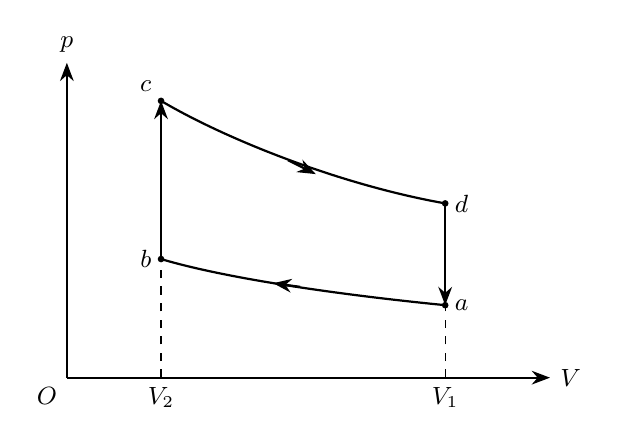
\begin{tikzpicture}[x=1.04cm,y=0.93cm,>=Stealth,every node/.style={font=\small}]
  \draw[->,thick] (0,0)--(5.9,0) node[right] {$V$};
  \draw[->,thick] (0,0)--(0,4.30) node[above] {$p$};
  \node[below left] at (0,0) {$O$};
  \coordinate (b) at (1.15,1.62); \coordinate (c) at (1.15,3.78);
  \coordinate (a) at (4.62,0.99); \coordinate (d) at (4.62,2.38);
  \draw[thick,->] (b)--(c);
  \draw[thick] (c)..controls (2.0,3.22) and (3.4,2.62)..(d);
  \draw[->,thick] (2.70,2.97)--(3.04,2.78);
  \draw[thick,->] (d)--(a);
  \draw[thick] (a)..controls (3.35,1.13) and (1.96,1.35)..(b);
  \draw[->,thick] (2.85,1.24)--(2.52,1.29);
  \draw[dashed] (1.15,0)--(1.15,1.62) (4.62,0)--(4.62,0.98);
  \foreach \name/\pos in {b/left,c/above left,a/right,d/right}{\fill (\name) circle(1.2pt) node[\pos] {$\name$};}
  \node[below] at (1.15,0) {$V_2$};
  \node[below] at (4.62,0) {$V_1$};
\end{tikzpicture}
\end{compactfigure}
\begin{enumerate}[label=\arabic*)]
\item 此循环中哪些过程，气体的温度升高？
\item 若 $V_1=5V_2$，求此循环的效率 $\eta$。（写成推导过程，结果保留三位有效数字。）
\end{enumerate}

\qitem{5.（4 分）}绳上有沿 $z$ 轴传播的横波，其波函数为 $\psi_1=A\cos\bigl(\omega t+2\pi z/\lambda\bigr)$，其中 $A$、$\omega$ 和 $\lambda$ 为已知常量。若此波在 $z=-L$（$L>0$）处发生反射，反射点为固定端，且反射时无能量损失。求：
\begin{enumerate}[label=\arabic*)]
\item 反射波的波函数 $\psi_2$；
\item 合成波（入射波和反射波的叠加）的各波节位置。
\end{enumerate}

\needspace{9\baselineskip}\noindent\textbf{判断题（原稿第 3 页）}\quad 在括号内判断正误。
\begin{enumerate}[label=\arabic*.,leftmargin=2.3em]
\item 同一系统经历不同的热力学过程，热容是一样的。\tfbox
\item 系统的热容不可能为负。\tfbox
\item 系统的热容可能为零。\tfbox
\item 准静态过程一定是可逆过程。\tfbox
\item 在封闭系统内发生的一切热力学过程系统的熵永不减小。\tfbox
\item 系统经历任一不可逆循环的熵变一定为零。\tfbox
\item 系统经历任一可逆过程的熵变一定为零。\tfbox
\item 一切与热现象有关的实际宏观过程都是不可逆过程。\tfbox
\item 制冷机的制冷系数一定小于 $1$。\tfbox
\item 气体的温度是大量气体分子热运动的集体表现，具有统计意义。\tfbox
\item 一平面简谐纵波在弹性介质中传播时，介质中各质元的振动动能和弹性势能在任一时刻相等。\tfbox
\item 对于作简谐振动的单摆，小球绕悬挂点的角速度是它振动的角频率。\tfbox
\end{enumerate}

\sourcepage{4}
\qitem{2.（3 分）}用绝热材料制成的一个容器，体积为 $2V_0$，被绝热板隔成 $A$、$B$ 两部分。$A$ 内储有 $1\,\mathrm{mol}$ 单原子分子理想气体，$B$ 内储有 $2\,\mathrm{mol}$ 刚性双原子分子理想气体，$A$、$B$ 两部分压强均为 $p_0$，两部分体积均为 $V_0$。设摩尔气体常量为 $R$。若抽去绝热板，两种气体混合后处于平衡时的温度 $T$ 为 $\fillblank[4.5cm]$。

\end{document}